\chapter{Background}\label{chap:background}
The upcoming chapter gives a basic description of electric grids and their structure. Afterwards, the functionality of Ant Colony Optimization (ACS) and its application to grid planning is presented. The goal is to provide sufficient background information for the understanding of the presented algorithm and its evaluation (i.e. for scholars of computer science or mathematics without previous knowledge about electric grids).

\section{Electric Grids}
An electric grid is the infrastructure, which enables the distribution of electric energy. Important components of a grid are the following.

\subsection{Components}\label{sec:components}

\textbf{Sources}: At sources electricity is fed into the electric grid (power plants, wind turbines, solar-panels etc.).

\textbf{Loads}: At loads electricity is subtracted (households, factories etc.).

\textbf{Lines}: Transmission lines which connect sources and loads and transport the electricity.

\textbf{Buses}: A bus is a connection point between two lines or more. Loads and sources can be coupled to a bus but it can also be a mere connection point.

\textbf{Transformers}: Transform the voltage from one voltage level to another one. A transformer therefore can also be seen as a generator or source within a certain voltage level. It functions as a connection between the different voltage levels of the grid.

\textbf{Switches}: Enable the opening and closing of connections between different branches of the grid. They are used cut off electricity from a branch in case of an emergency or to supply electricity to the consumer via an alternative route (n-1 criterion).

\textbf{Storage Units}: Enable the storage of energy (via pumped storage hydroelectricity, batteries, hydrogen etc.). 


\textbf{Transformers}: Transform the voltage from one voltage level to another one. A transformer therefore can also be seen as a generator or source within a certain voltage level.

\subsection{Structure}
To increase efficiency, the grid is usually separated into three different voltage levels: high-(HV), medium-(MV) and low-voltage (LV).

\textbf{HV grids} connect big power plants and transformer stations of underlying medium-voltage (MV) grids. They usually operate at voltages reaching from 110 to 380 kV. Their structure is more meshed to build up redundancy for safety.

\textbf{MV grids} connect smaller power plants, factories and transformer stations to the low-voltage (LV) level. They operate at around 10 to 20 kV and are required to fulfill the n-1 criterion. So if one component of the MV grid fails, there is at least one built in redundancy to keep the grid functional.

\textbf{LV grids} mostly transfer electricity from the transformer stations to the households. Due to the increasing decentralized feedin of electricity the MV grid also needs to be capable of transferring energy between households. They usually operate at voltages of around 0.4k V.

\begin{figure}[h]
	\begin{centering}
		{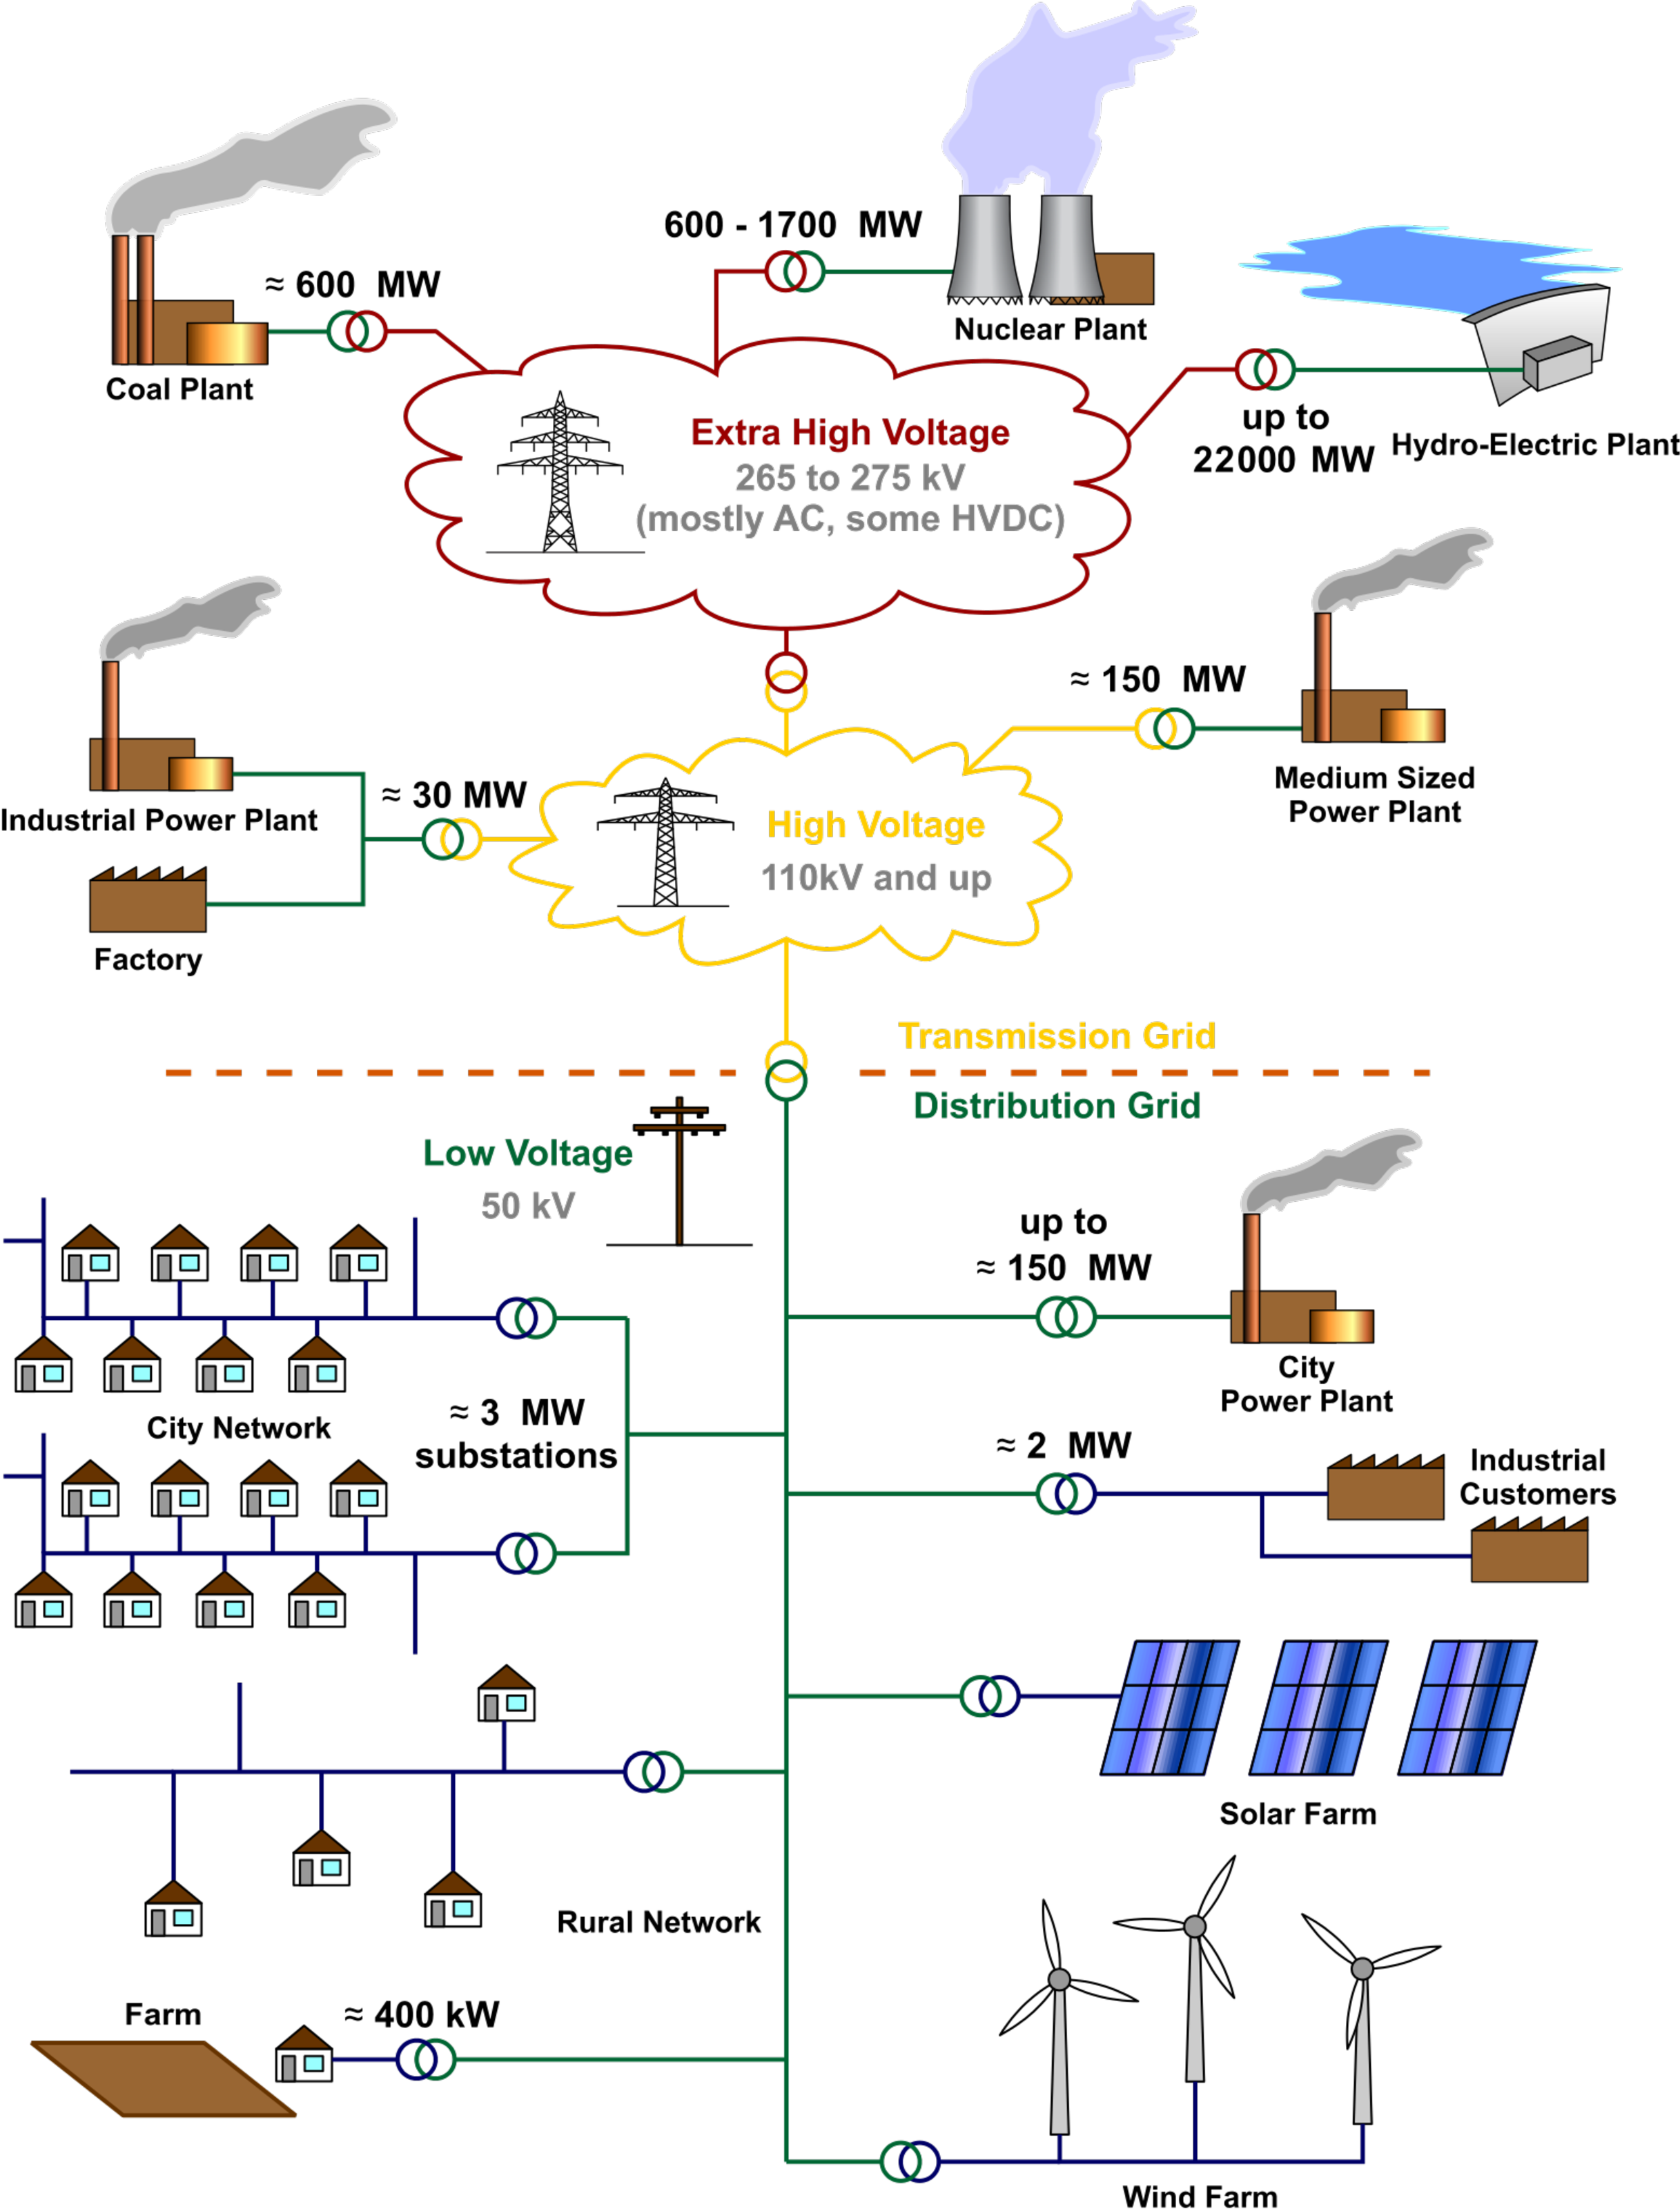
\includegraphics[scale=0.27]{figures/background/grid_schematic.pdf}}
		\caption{Schematic depiction of the electricity grid common in Germany.}
		\label{fig:tri}
	\end{centering}
\end{figure}

%TODO: put in source of figure!
% https://commons.wikimedia.org/wiki/File:Electricity_Grid_Schematic_English.svg


\section{Ant Colony Optimization}
ACO is inspired by the astonishing ability of real ants to find short paths between their nest to sources of food. Ants are mostly blind and coordinate their movements using pheromones, which they leave behind on their trails. Ants are able to sense the pheromones and tend to follow paths with a higher concentration of the messenger substance. Ants which probabilistically follow the paths with higher pheromone concentration again leave behind pheromones which increase the chance of other ants to also follow this trail. Over time, this leads to a convergence of ants to follow the path with the highest pheromone concentration.

\subsection{The Double Bridge Experiment}

The following example is based on experiments Deneubourg et al. \cite{deneubourg1990self} conducted with Argentine ants in 1990. The ants are placed at the starting location and two paths of different length connect them to a source of food.
\begin{figure}[h]
	\begin{centering}
		{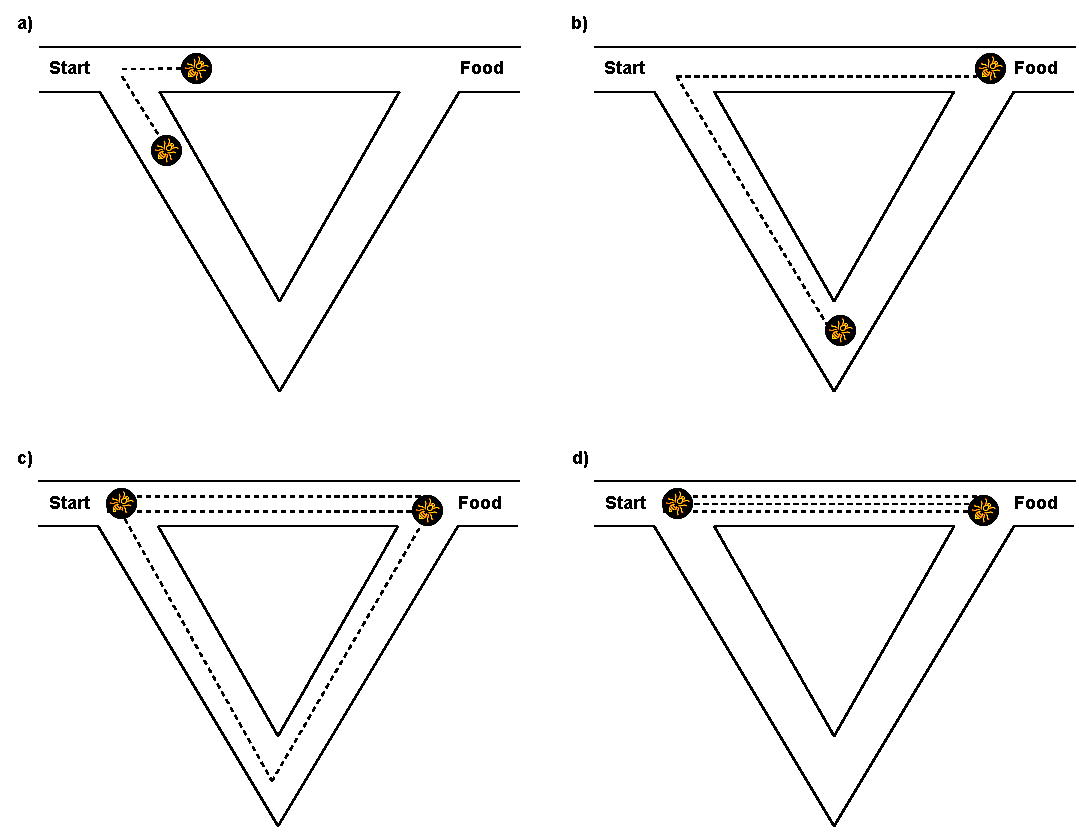
\includegraphics[scale=0.8]{figures/background/aco_double_bridge.pdf}}
		\caption{Double Bridge Experiment. Two paths of different length lead from the start to the food source.}
		\label{fig:double_bridge}
	\end{centering}
\end{figure}

As shown in \ref{fig:double_bridge}, at the beginning of the experiment the ants decide randomly which path they chose, since no pheromone has been distributed yet (a). Because one path is shorter, the ants who chose this path arrive at the food source earlier (b). On the way back, there only exists pheromone on the shorter path, which leads to a higher chance of ants choosing it (c). Over time, this leads to the convergence of most ants following the short path (d).

In general, ants do not deterministically follow the path with the highest pheromone concentration, but just with a higher chance. This means, that there is still the possibility of an ant to chose a different path and explore new routes. Thereby, new sources of food or potentially even shorter routes can be discovered. Just the discovery of new short paths alone does not suffice to bring the majority of ants to switch to it. In the real world, but also for ACO the pheromone is evaporating over time, which leads to the "forgetting" of old established paths. On shorter paths, the ants refresh the pheromones more quickly, which increases the chance for more ants to chose them. The non deterministic behavior and the evaporation of pheromones together make it possible for ants to adapt to new situations.

\subsection{Model}
To model the behavior of real ants finding the shortest path Dorigo and Stützle \cite{DBLP:books/daglib/0013523} suggest using a simple graph model on which the ants can traverse edges from one node to the next. In the case of the double bridge experiment three nodes (Start, Food, Way) and three edges connecting the nodes are needed to adequately model the location (see Figure \ref{fig:double_bridge_graph}). Another simplification for the model is to discretize time into times-steps $t = 1,2,3,...$.
\begin{figure}[h]
	\begin{centering}
		{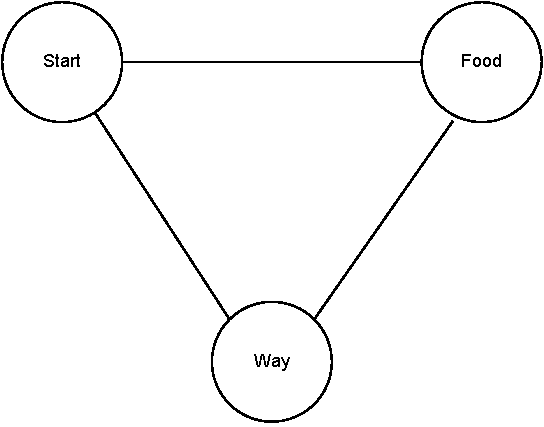
\includegraphics[scale=0.5]{figures/background/double_bridge_graph.pdf}}
		\caption{Model of the Double Bridge Experiment as a graph. The long branch consists of two edges (Start, Way), (Way, Food)}
		\label{fig:double_bridge_graph}
	\end{centering}
\end{figure}

Now $p_{is}(t)$ describes the probability that an ant at time $t$ at location $i$ chooses the short path $s$ and $p_{is}(t)$ the long path $l$. To define these probabilities the pheromone level $\varphi_{ia}$ an ant encounters at node $i\in{(Start,Food)}$ on branch $a \in {(l, s)}$ has to be considered. The long branch $l$ is exactly two times longer than the short branch $s$ and therefore also take two time-steps to traverse instead of one. This leads to the following equations:
$$p_{is}(t) = \frac{[\varphi_{is}(t)]^\alpha}{[\varphi_{is}(t)]^\alpha + [\varphi_{il}(t)]^\alpha}, \;p_{il}(t) = \frac{[\varphi_{il}(t)]^\alpha}{[\varphi_{is}(t)]^\alpha + [\varphi_{il}(t)]^\alpha},$$
where $p_{is}(t) + p_{il}(t) = 1$ and $\alpha$ is a parameter. The update of pheromones on the two branches is described as:
$$\varphi_{is}(t) = \varphi_{is}(t-1) + p_{is}(t-1)m_i(t-1) + p_{js}(t-1)m_j(t-1),$$
$$(i = Start, j = Food; i = Food, j = Start),$$
$$\varphi_{il}(t) = \varphi_{il}(t-1) + p_{il}(t-1)m_i(t-1) + p_{jl}(t-2)m_j(t-2),$$
$$(i = Start, j = Food; i = Food, j = Start),$$
where $m_i(t)$, the number of ants at node $i$ at time $t$ is given by:
$$m_i(t) =  p_{js}(t-1)m_j(t-1) + p_{jl}(t-2)m_j(t-2),$$
$$(i = Start, j = Food; i = Food, j = Start),$$
\cite{DBLP:books/daglib/0013523} show, that simulations with $\alpha = 2$ lead to a quick convergence of the ants towards the use of the short branch.\\
To expand the described system to find shortest paths in more complex graphs requires the ants to additionally receive a small memory. This enables them to avoid loops and to remember the entire solution they built. They can then evaluate the built solution to determine the quantity of pheromone to deposit. As mentioned before, the performance can be greatly improved by adding evaporation to the pheromones.

\subsection{General Ant Colony Optimization}
To solve more general minimum cost problems on graphs ACO performs two main steps being the \textbf{solution construction} and the \textbf{evaluation}.\\
Firstly, a solution is constructed by an ant beginning at the starting node and incrementally adding neighboring nodes. The decision which node to add next is influenced by pheromones deposited in previous iterations. In the very first iteration the pheromone is uniformly distributed along the paths and the decision rule is therefore random. Additionally, a heuristic function $\eta$ can be used to find better results faster. A common heuristic for short paths is the inverse of the euclidean distance to the destination. Using a heuristic is a greedy approach and a balance between learning via pheromones and preset knowledge via heuristics is crucial. This procedure is repeated until the destination node is reached. Note, in case of grid planning a solution requires all nodes to be added. The order of how the nodes are added and over which edges is stored in memory.
The probability of an ant choosing path $i$ considering the heuristic can be formalized in the following way:
$$p_i = \frac{\varphi_i^\alpha\eta_i^\beta}{\sum_{j\in{w}}\varphi_j^\alpha\eta_j^\beta},$$
where $w$ is the set of all paths reachable from the current position and $i,j \in w$. $\varphi_i$ is the amount of pheromone on path $i$ and $\eta_i$ is the heuristic value on path $i$. $\alpha$ and $\beta$ are parameters to determine the relation of pheromones and heuristics in the decision of the ant. Furthermore, it holds $\sum_{k\in{w}}p_k = 1$. \\
Secondly, the build solution is evaluated and its cost is calculated. Now the amount of pheromone this particular solution should receive is set according to the cost. This could for example be the inverse of the solutions cost. Thereby, solutions with low cost receive more pheromones and vice versa. In the next iteration, the pheromone deposited from the previous solution influences the way in which new nodes are added. Pheromone evaporation can help to reduce the weight that older solutions have on the pheromone level where less information about the problem existed. Generally, more evaporation leads to more exploration of the search space. Evaporation also helps to bound the maximal amount of pheromone achievable. Update and evaporation can be formulated in the following way:
$$\varphi_i = (1-p)\varphi_i + p\Delta\varphi_i$$
$$\text{with } \Delta\varphi_i = \begin{cases}
	1 & \, \text{if i is part of solution}\\
	0 & \, \text{else}
\end{cases}$$
where $p$ is the evaporation factor and $\varphi_i$ is the amount of pheromone deposited on path i.
A detailed description of the presented ACO algorithm Ant-Power-Medium-Voltage will be presented in section \ref{sec:antpowermv}.


\section{ACO In Grid Planning}

To bring ACO and grid planning together, one needs to formulate the grid planning problem in a way so it can be solved by an ACO algorithm. A suitable way to do this, is to use graphs as a model of the electric grid. Intuitively, the buses of the grid can be seen as nodes (sources, loads are transformers are directly coupled to the buses), whereas the transmission lines connecting the buses are the edges. Let $G = (B, E)$ be an undirected graph, where the nodes $B$ are the buses $b_1, b_2, ...$ of the grid and the edges $E$ resemble the transmission lines $t_1, t_2, ...$. The goal is to build a graph, where all nodes are connected at the lowest cost possible. Additional constraints like the topology of the graph also have to be considered. As long as the graph is well defined the ACO algorithm can operate in a similar way as previously shown.
The node which represents the transformer connecting the grid to the overlying voltage level is used as a starting point. It serves as a source to the other buses electricity demand. At the start, none of the nodes are connected to each other and incrementally edges (transmission lines) are added to the graph until all nodes are connected through a path to the starting node (transformer). Afterwards, the cost of such a solution is calculated and the pheromone update is performed on the used paths accordingly.

\subsection{Delaunay Triangulation}\label{triangulation}
Theoretically, every network station could be connected with all other stations, which is infeasible in practice due to economic reasons. But also for computing, a reduction of the number of potential connections between network stations reduces the algorithms runtime exponentially (reduction of the search space). The Delaunay triangulation is a suitable method to reduce the number of potential lines between stations. It divides a surface with points into triangles by maximizing the minimum of all the angles of the triangles in the triangulation.
\begin{figure}[h]
	\begin{centering}
		{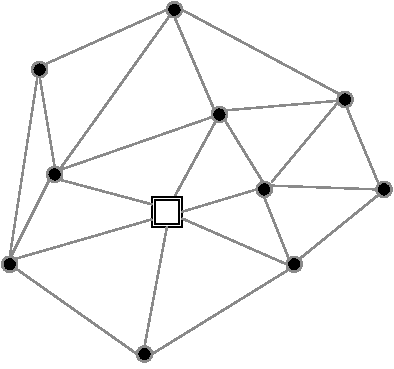
\includegraphics[scale=0.7]{figures/background/tri.pdf}}
		\caption{Delaunay Triangulation of a set of buses and a transformer.}
		\label{fig:tri}
	\end{centering}
\end{figure}

An example of this can be seen in Figure \ref{fig:tri} where the transformer is marked with a square. Research shows, that for the related TSP only 1\% of the edges belong to the optimal solution and are not part of the triangulation \cite{schmitting2000traveling}. The exponential reduction of the number of connections between $N$ buses can be shown via the following equations:
$$e_{total} = \frac{1}{2}N(N-1)\text{ versus }e_{tri} = 3N - 3 - N_h$$
where $e_{total}$ is the number of all possible connections and $e_{tri}$ is the number of possible connections after applying the triangulation. $N_h$ is the number of nodes being part of the convex hull. \\

\subsection{Ant Graph}\label{ant_graph}
The triangulation can additionally be used to create a new graph called ant graph which simplifies the mathematical formulation of the ring network planning problem \cite{rotering2013zielnetzplanung}. To build this graph, the incenter of the triangles and the transformer are taken as nodes. Edges are created between triangles which share a common side. Since every triangle already constitutes a ring in itself using them to built a solution which satisfies the topological constraints is very helpful. If a neighboring ant node (triangle) is added, the hull of the represented triangles again forms a ring. As long as this ring contains the transformer as a node a valid ring network design is produced. An example is shown in Figure \ref{fig:aco_grid} where the unfilled circles represent the ant nodes and the dotted line the ant path.

\begin{figure}[h]
	\begin{centering}
		{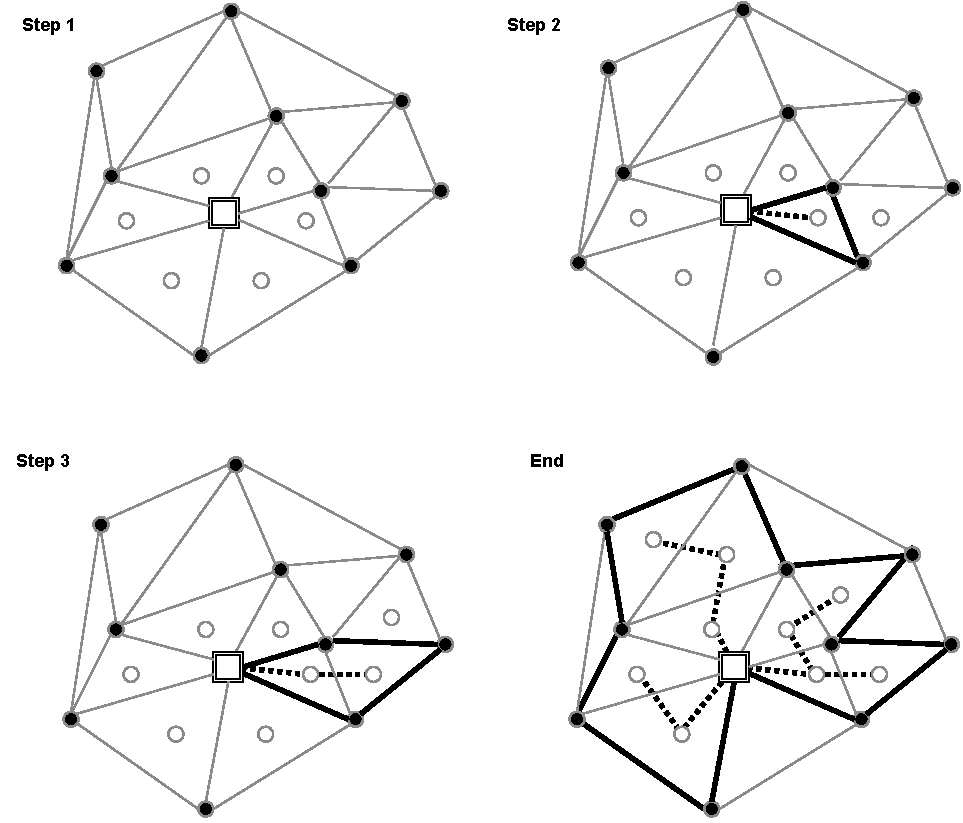
\includegraphics[width=\textwidth]{figures/background/aco_grid.pdf}}
		\caption{Building a solution on the ant graph.}
		\label{fig:aco_grid}
	\end{centering}
\end{figure}

The expansion is started at the transformer (square). In step 1 no nodes are added to the transformer. The first expansion options are its neighboring ant nodes. After the first node is added in step 2, a new expansion option is accessed. The two stations (filled circles) together with the transformer already represent a valid ring network structure. In step 3 a second triangle is added so the hull of the two triangles is the new intermediate ring network solution. This procedure is repeated until all stations are covered by the triangles represented by ant nodes.


%TODO: add source, why delaunay is suitable for grids page 65 Rotering [155]
%TODO: add source shortest paths lie to 99\% on triangulation. [155]



